\section{Processi primari}\label{ProcessiPrimari}

    \subsection{Processo di fornitura}\label{PP:Fornitura}	%istanziare Management Process, Infrastructure Process e Improvement Process

        \subsubsection{Scopo}\label{PP:Fornitura:Scopo}
		La sezione corrente ha lo scopo di riportare le attività principali che impegneremo ad attuare al fine di
		diventare \gloss{fornitori} per la proponente \II.

		\subsubsection{Ricerca delle tecnologie}
		Ognuno di noi approfondirà la propria conoscenza su tecnologie e \gloss{framework} vari, in modo da discutere insieme quali sono
		quelle di interesse comune e di utilità per il progetto. Questo prevede poi l'auto-formazione di quelle scelte in comune accordo
		per acquisirne una buona padronanza.

		\subsubsection{Normazione}\label{Normazione}
		L'attività di normazione prevede l'incremento del documento corrente ogni qual volta lo si ritiene necessario.
		Essendo infatti un documento incrementale, è possibile che vengano aggiunte delle nuove regole o aggiornate quelle già presenti.
		Facendo un esempio: arrivati al momento di riscrittura dei casi d'uso, dopo la prima revisione, abbiamo dovuto suddividere i casi in categorie ben distinte, in modo che fosse evidente il sottosistema di riferimento di Butterfly.
		Di conseguenza, cambiare il codice identificativo di ognuno e cambiare la relativa norma nel paragrafo \S\ref{PP:Sviluppo:AdR:CasiUso}.

        \subsubsection{Studio di fattibilità}\label{PP:Fornitura:SdF}
        In quest'attività viene prodotto il documento \Doc{\SdFv} al fine di analizzare ogni \gloss{capitolato} e scegliere quale contratto accettare.
        Nello specifico, il documento in ogni sezione contiene:
        	\begin{itemize}
        		\item \textbf{Descrizione generale}: breve descrizione del capitolato.
        		\item \textbf{Obiettivo finale}: obiettivo da raggiungere.
        		\item \textbf{Tecnologie coinvolte}: elenco delle tecnologie direttamente coinvolte esplicitate nel capitolato.
        		\item \textbf{Valutazione conclusiva}: giudizio finale del team di sviluppo.
        	\end{itemize}

        \subsubsection{Preparazione in vista della revisione}
		In questa attività prepariamo tutto il materiale necessario per il buon superamento della revisione:
		\begin{itemize}
			\item I vari documenti, i verbali e la lettera di presentazione per quanto riguarda la documentazione in ingresso
			\item I diagrammi dei package e il codice necessario per la realizzazione del \gloss{Proof of Concept}
			\item Le diapositive per l'esposizione
		\end{itemize}

    \subsection{Processo di sviluppo}\label{PP:Sviluppo}

		\subsubsection{Scopo}\label{PP:Sviluppo:Scopo}
		Lo sviluppo consiste nell'affrontare le attività volte a produrre il software richiesto dal proponente.
		Per una corretta implementazione di questo \gloss{processo}, è necessario:
		\begin{itemize}
			\item Fissare degli obiettivi di sviluppo
			\item Realizzare un prodotto che sia conforme a:
			\begin{itemize}
				\item \gloss{Requisiti} definiti dal proponente
				\item Test definiti dalle norme di \gloss{qualità}
			\end{itemize}
		\end{itemize}
		Lo standard ISO/IEC 12207:1995\footnote{Riferirsi alla voce ``ISO/IEC 12207'' in \S\ref{rifnorma}} definisce il processo di
		sviluppo quel processo contenente tutte le attività relative al prodotto finale, quali:
		\begin{itemize} % [noitemsep]
			\item Analisi dei requisiti
			\item Progettazione
			\item Codifica
			\item Integrazione ed installazione
		\end{itemize}


        \subsubsection{Analisi dei requisiti}\label{PP:Sviluppo:AdR}
		Gli Analisti si occupano di redigere l'\Doc{\AdRv}, composta come segue:
		\begin{itemize}
			\item Descrizione generale del prodotto
			\item Modellazione concettuale del \gloss{sistema} tramite la definizione dei vari \gloss{casi d'uso}
			\item Classificazione e tracciamento dei requisiti
		\end{itemize}

		\paragraph{Denominazione dei requisiti}\label{PP:Sviluppo:AdR:DenominazioneRequisiti}
		Ogni requisito che è stato individuato durante l'analisi presenta il seguente identificativo univoco:
		\begin{center}
			\texttt{R[Numero][Tipo][Priorità]}
		\end{center}

		\begin{itemize}
			\item \textbf{R}: si riferisce a requisito.
		 	\item \textbf{Numero}: corrisponde ad un numero che cerca di seguire la struttura del documento ed è progressivo. Inizia da 1.
		 	\item \textbf{Tipo}: segnala la tipologia di requisito che può essere di:
		 	\begin{itemize}
		 		\item \textbf{F}: funzionalità, che ha a che vedere con le funzionalità del sistema software.
		 		\item \textbf{Q}: qualità, che riguarda tecniche ad hoc.
		 		\item \textbf{V}: vincolo, proposto da \II.
		 	\end{itemize}
	 		\item \textbf{Priorità}: indica il grado di urgenza per il soddisfacimento di un requisito, come:
	 		\begin{itemize}
	 			\item \textbf{0}: opzionale, di grado basso e solo marginalmente utile.
	 			\item \textbf{1}: desiderabile, di medio livello quindi non strettamente necessario ma che dà valore aggiunto.
	 			\item \textbf{2}: obbligatorio, di grado alto quindi irrinunciabile per il \gloss{committente} e impossibile da tralasciare.
	 		\end{itemize}
		\end{itemize}

		Esempio: \texttt{R2Q1} indica il secondo requisito di qualità ed è desiderabile.


		\paragraph{Metriche sui requisiti}\label{MetricheAdR}
		Dato che non è fisso il numero dei requisiti di un progetto, abbiamo scelto una serie di metriche dove il valore ottimale da raggiungere è sempre uguale, lo zero. Abbiamo anche scelto di contare il numero di requisiti non soddisfatti invece che il contrario. Lo stesso ragionamento è valido per quanto	riguarda i rischi che possono verificarsi nel corso del progetto.
		Gli obiettivi che si vogliono raggiungere attraverso tali metriche possono essere stabiliti solo a progetto concluso.

		La denominazione delle metriche è descritta in \S\ref{Classificazione metriche}.

		\subparagraph{MPR005 Requisiti obbligatori non soddisfatti}
		Per adempiere completamente alla richiesta del cliente, ci serve individuare tutti i requisiti presenti nella sua richiesta, impliciti, espliciti, diretti e derivati. Alcuni sono imprescindibili, detti obbligatori, e il loro soddisfacimento determina la buona riuscita del progetto.

		\textbf{Metrica}: numero dei requisiti obbligatori non soddisfatti.

		\subparagraph{MPR006 Requisiti desiderabili non soddisfatti}
		I requisiti desiderabili non sono necessari, ma offrono un valore aggiunto al progetto.

		\textbf{Metrica}: numero dei requisiti desiderabili non soddisfatti.

		\subparagraph{MPR007 Requisiti opzionali non soddisfatti}
		Tali requisiti dovranno essere adempiuti solo nel momento in cui tutti i requisiti obbligatori saranno soddisfatti.
		Possono essere concordati col cliente in corso d'opera.

		\textbf{Metrica}: numero dei requisiti opzionali non soddisfatti.


		\paragraph{Casi d'uso}\label{PP:Sviluppo:AdR:CasiUso}
		Un caso d'uso è una tecnica che identifica i requisiti funzionali descrivendo le interazioni tra il sistema di riferimento e un utente ad esso esterno.\par
		Ogni caso d'uso che si vuol descrivere presenta:
		\begin{itemize}
		 	\item \textbf{Codice}: per l'identificazione.
		 	\item \textbf{Titolo}: denominazione del caso d'uso, possibilmente breve.
		 	\item \textbf{Attori primari}: tutti gli \gloss{attori} primari coinvolti.
		 	\item \textbf{Attori secondari}: opzionale, tutti gli attori secondari coinvolti.
		 	\item \textbf{Descrizione}: per spiegare più nel dettaglio le azioni che vengono compiute.
		 	\item \textbf{Precondizione}: per rappresentare lo stato del sistema nell'istante precedente.
		 	\item \textbf{Postcondizione}: per rappresentare lo stato del sistema l'istante successivo.
		 	\item \textbf{Scenario principale}: contenente la serie di azioni da compiere numerate nell'ordine in cui vengono compiute.
		 	\item \textbf{Estensioni}: opzionale, per azioni inerenti a scenari alternativi come d'eccezione o errore.
		\end{itemize}

		\subparagraph{Denominazione del codice identificativo}
		Ogni codice presenta una forma del tipo:
		\begin{center}
			\texttt{UC[Numero]-[Sottosistema]}
		\end{center}

		\begin{itemize}
			\item \textbf{UC}: sta per "User Case", l'equivalente inglese di "caso d'uso".
			\item \textbf{Numero}: numero progressivo che si riferisce al caso. Se il caso d'uso è principale, è un semplice intero (e.g. 1 per il primo caso d'uso). Mentre se è un sotto caso, presenta due interi separati da un punto (e.g 1.1 per per il primo figlio del primo caso d'uso).
			\item \textbf{Sistema}: indica il sistema preso come riferimento per il caso d'uso, che può essere Butterfly o un suo sottosistema:
			\begin{itemize}
				\item \textbf{PR}: Producer Redmine.
				\item \textbf{PG}: Producer Gitlab.
				\item \textbf{GP}: Gestore Personale.
				\item \textbf{CT}: Consumer Telegram.
				\item \textbf{CE}: Consumer Email.
				\item \textbf{BT}: bot Telegram.
				\item \textbf{SE}: server Email.
			\end{itemize}
		\end{itemize}

		Vi possono essere al massimo tre livelli di annidamento, come nel seguente esempio:
		\begin{itemize}
			\item \texttt{UC1} identifica il caso d'uso con il numero 1
			\item \texttt{UC1.1} identifica il sottocaso 1 del caso d'uso 1
			\item \texttt{UC1.1.1} identifica il sottocaso 1 del caso d'uso 1.1
		\end{itemize}
		Per ogni livello i numeri partono da 1.

        \subsubsection{Progettazione}\label{PP:Sviluppo:Progettazione}
        La progettazione è l'attività svolta dai progettisti con il fine di dare una soluzione soddisfacente per tutti gli stakeholder coinvolti nel rispetto delle best practice e dei design pattern scelti, attraverso la descrizione dell'architettura del software.

		\paragraph{Obiettivi}\label{PP:Sviluppo:Progettazione:Obiettivi}
        Gli obiettivi dell'attività di progettazione sono:
        \begin{itemize}
			\item Definire l'architettura logica del prodotto.
			\item Organizzare le responsabilità di realizzazione.
			\item Garantire la qualità del prodotto finale.
		\end{itemize}


		\subsubsection{Diagrammi UML}\label{PP:Sviluppo:UML}

		\paragraph{Diagrammi delle classi}\label{PP:Sviluppo:DiagrammiClassi}
		Per i diagrammi delle classi utilizziamo lo strumento \gloss{Draw.io} e il linguaggio \gloss{UML} 2.0.\par
        Questi diagrammi strutturali descrivono ad alto livello i tipi di oggetto presenti nel sistema e le relazioni che intercorrono tra essi.
		I diagrammi delle classi sono composti dalle seguenti proprietà:
		\begin{itemize}
			\item \textbf{Attributi}: rappresentano lo stato dell'oggetto. Presentano le caratteristiche:
			    \begin{itemize}
			        \item \textbf{Visibilità}: pubblica (+), privata(-) o protetta(\#) rispetto alle altre classi.
			        \item \textbf{Nome}: nome dell'attributo.
			        \item \textbf{Tipo}: tipo dell'attributo (intero, stringa\dots).
			        \item \textbf{Molteplicità}: numero di occorrenze dell'attributo (opzionale).
			        \item \textbf{Default}: valore di default dell'attributo (opzionale).
                    \item \textbf{Altro}: molteplicità\dots (opzionali)
			    \end{itemize}
			\item \textbf{Associazioni}: rappresentano legami tra classi.\par
                        Le rappresentiamo con linee continue orientate tra due classi, hanno un nome.
		\end{itemize}
        Nella parte bassa del rettangolo delle classi rappresentiamo le operazioni fornite dalla classe, composte da:
        \begin{itemize}
            \item \textbf{Visibilità}: come per gli attributi.
            \item \textbf{Nome}: nome dell'operazione.
            \item \textbf{Lista dei parametri}: parametri necessari all'operazione. Sono formati da:
            \begin{itemize}
                \item \textbf{Direzione}: indica se il parametro è in lettura (in), scrittura (out) o entrambi (inout). Opzionale, di default è in lettura.
                \item \textbf{Nome}: nome del parametro.
                \item \textbf{Tipo}: tipo del parametro.
                \item \textbf{Default}: valore di default del parametro (opzionale).
            \end{itemize}
            \item \textbf{Tipo di ritorno}: tipo ritornato dall'operazione.
        \end{itemize}
        Tra le classi rappresentiamo le seguenti relazioni di dipendenza:
        \begin{itemize}
            \item \textbf{Dipendenza}: rappresentata da una linea orientata tratteggiata, indica che una classe usa un'operazione fornita dalla classe puntata.
            %TODO: la mettiamo? \item \textbf{Associazione}: rappresentata da una linea continua semplice, indica che una classe possiede uno o più attributi (a seconda delle molteplicità indicate sulla linea) dell'altra, o viceversa.
            \item \textbf{Aggregazione}: rappresentata da un diamante vuoto seguito da una linea continua, indica che una classe (puntata dal diamante) possiede un'istanza di un'altra classe tra gli attributi. Tale istanza può essere condivisa.
            \item \textbf{Composizione}: rappresentata da un diamante pieno seguito da una linea continua, è come l'aggregazione ma in tal caso l'aggregato non è condiviso tra più istanze.
            \item \textbf{Generalizzazione}: rappresentata da una freccia vuota, indica che ogni classe che punta verso un'altra è anche un'istanza di essa (eredita metodi e attributi).
        \end{itemize}
        Usiamo inoltre i seguenti costrutti:
            \begin{itemize}
                \item \textbf{Classi astratte}: il nome è indicato in corsivo, non possono essere istanziate. Presentano almeno un'operazione astratta (con il nome in corsivo) e possono avere attributi.\par
                Tali classi generalizzano altre classi che devono implementare le operazioni astratte per essere istanziate, altrimenti sono anch'esse astratte e generalizzano altre classi.
                \item \textbf{Interfacce}: indicate da un pallino vuoto e una linea continua verso classi, presentano solamente le operazioni che vengono implementate dalle classi collegate con la linea.\par
                Possono essere indicate con un pallino vuoto e un semicerchio a destra per indicare che l'interfaccia viene usata da un componente in un punto qualsiasi (ritorno di un'operazione, attributo\dots).
            \end{itemize}

		%\subparagraph{Semantica} %TODO
		%Dipendenza generica, Associazione, Aggregazione..
        %Meglio qui o lasciamo sopra?

        \paragraph{Diagrammi dei package}\label{PP:Sviluppo:DiagrammiPackage}
        Per i diagrammi dei package utilizziamo lo strumento \gloss{Draw.io} e il linguaggio \gloss{UML} 2.0.\par
        Vengono usati insieme ai diagrammi delle classi per raggrupparne gli elementi in un elemento di livello più alto.
        Rappresentiamo i package con un rettangolo che contiene altri package o classi, e un'etichetta con il nome del package.
        Ogni package identifica uno spazio dei nomi, che serve per dare un nome qualificato alle classi.
        Gli elementi di un package possono avere visibilità pubblica(+) o privata(-) verso l'esterno.
		Nella progettazione adottiamo il principio del common closure principle, secondo il quale elementi dello stesso
		package condividono la stessa causa di cambiamento.
        Indichiamo le dipendenze tra package con frecce tratteggiate.
        Rappresentiamo le dipendenze perché:
        \begin{itemize}
            \item Individuiamo subito le dipendenze circolari, evitandole
            \item Vediamo quali elementi dovrebbero essere più stabili (avendo più dipendenze entranti)
        \end{itemize}


		\paragraph{Diagrammi di attività}\label{PP:Sviluppo:DiagrammiAttività}
        Per i diagrammi di attività utilizziamo lo strumento \gloss{Draw.io} e il linguaggio \gloss{UML} 2.0.\par
		Li usiamo per descrivere la logica dell'applicazione, ovvero quali attività si possono presentare e in quali sequenze vengono svolte. Rappresentano quindi la parte dinamica dei casi d'uso.\par
        Le attività sono insiemi di azioni ordinate dei tipi:
        \begin{itemize}
            \item \textbf{Nodo iniziale}: rappresentato da un pallino pieno, è l'inizio dell'attività.
            \item \textbf{Fork}: rappresentato da un tratto marcato, indica l'inizio di elaborazioni parallele.
            \item \textbf{Join}: rappresentato da un tratto marcato, indica un punto di sincronizzazione tra elaborazioni parallele.\par
                Vengono indicate specifiche di join tra parentesi quadre (espressioni booleane).
            \item \textbf{Branch}: rappresentato da un rombo vuoto, indica che si può intraprendere solo uno dei possibili percorsi.
            \item \textbf{Merge}: rappresentato da un rombo vuoto, è simile alla join. Differisce per il fatto che unisce più possibili elaborazioni non parallele ma in alternativa tra esse, porvenienti da uno o più branch.
            \item \textbf{Pin parametro}: rappresentati da box, sono parametri che rappresentano risorse prodotte da azioni e consumate da altre azioni.
            \item \textbf{Nodo finale}: rappresentato da un pallino pieno circondato da un cerchio, indica il termine dell'attività con successo.
            \item \textbf{Nodo di fine flusso}: rappresentato da un cerchio con una croce, non termina l'attività.\par
                Viene usata per casi speciali (eccezione, ramo del branch\dots).
        \end{itemize}
        Ogni attività può comporre un'azione. In tal caso si tratta di una sotto attività, e viene indicata con un simbolo a forca e da un rettangolo esterno con il nome dell'attività che ne rappresenta le azioni dall'input fino all'output.\par
        Usiamo inoltre i seguenti costrutti:
        \begin{itemize}
            \item \textbf{Swimlanes}: sono rappresentate da riquadri che suddividono la responsabilità delle azioni presenti nelle attività.\par
                Le azioni possono far capo a più swimlanes, per esempio l'azione di merge.
            \item \textbf{Segnali}: indicano eventi provenienti da processi esterni.\par
            Sono indicati in modo diverso a seconda dell'evento scatenante, che può essere dei seguenti tipi:
            \begin{itemize}
                \item \textbf{Eventi esterni}: l'evento generato viene rappresentato da un rettangolo con un lato a punta uscente, mentre l'azione che attende l'evento viene rappresentata con un rettangolo con un lato a punta entrante.
                \item \textbf{Eventi temporali}: viene rappresentato con una clessidra e ne viene indicato il tempo di ripetizione.\par
                    Può trovarsi all'inizio del flusso, sostituendo il nodo iniziale, per indicare che un'attività verrà eseguita ogni volta che l'evento temporale consuma il tempo indicato.
            \end{itemize}
        \end{itemize}
        %TODO verificare se parlare di flussi e archi
        Per indicare azioni che si ripetono su più elementi, ad esempio su una lista di elementi, usiamo le regioni di espansione.
        Le indichiamo con un rettangolo tratteggiato ad angoli arrotondati, e rettangoli piccoli presenti sui lati di inizio e fine regione, che rappresentano le liste di elementi processati.\par
        Le frecce di entrata e uscita indicano in quale verso viene svolta l'attività che include la regione di espansione.

		%\subparagraph{Semantica} %TODO
		%Ogni diagramma inizia con uno stato iniziale segnato con un pallino nero, ogni transizione è una freccia....


		\paragraph{Diagrammi di sequenza}\label{PP:Sviluppo:DiagrammiSequenza}
		Per i diagrammi di sequenza utilizziamo lo strumento \gloss{Draw.io} e il linguaggio \gloss{UML} 2.0.\par
        Usiamo questi diagrammi per descrivere come la collaborazione tramite messaggi di un gruppo di oggetti realizza un comportamento.\par
        Essi mostrano come gli oggetti interagiscono nel tempo, leggendo il diagramma dall'alto al basso.\par
        I principali costrutti usati sono:
        \begin{itemize}
            \item \textbf{Partecipanti}: rappresentati da un rettangolo contenente il nome dell'entità (spesso coincide col nome di una classe) e da una barra di attivazione (rettangolo che si prolunga per tutta la durata in cui l'entità è attiva), descrivono l'entità che detiene il flusso nel caso d'uso.
            \item \textbf{Messaggi}: rappresentano le operazioni chiamate tra le entità e i dati scambiati.\par
            Sono di diverse tipologie:
            \begin{itemize}
                \item \textbf{Sincroni}: rappresentati da una freccia piena con il nome del messaggio ed eventuali parametri tra parentesi tonde, descrivono la chiamata di un messaggio in cui l'entità chiamante attende la risposta dall'entità chiamata.
                \item \textbf{Asincroni}: rappresentati da una linea direzionata con il nome del messaggio ed eventuali parametri tra parentesi tonde, descrivono la chiamata di un messaggio in cui l'entità chiamante non attende la risposta dall'entità chiamata.
                \item \textbf{Ritorno}: rappresentati da una linea tratteggiata direzionata, indicano un messaggio di ritorno che risponde a un precedente messaggio di chiamata.
                \item \textbf{Creazione}: rappresentati da una linea tratteggiata direzionata e dalla notazione <<create>>, indicano la creazione di una nuova entità da parte dell'entità chiamante.
                \item \textbf{Distruzione}: rappresentati da una freccia piena e dalla notazione <<destroy>>, indicano la distruzione di un'entità da parte dell'entità chiamante.
            \end{itemize}
        \end{itemize}
        Per descrivere i cicli e le condizioni vengono utilizzati frame di interazione, rappresentati con un rettangolo che circonda i messaggi e le barre di attivazione coinvolte, con una label per indicare il tipo di frame, e da una guardia tra parentesi quadre nell'entità che ne scatena l'inizio.
        Vi sono i seguenti tipi di frame di interazione:
        \begin{itemize}
            \item \textbf{Alt}: più frame in alternativa, si sceglie in base alla guardia.
            \item \textbf{Opt}: opzionale, in base alla guardia si esegue o meno il frame.
            \item \textbf{Par}: parallelo, frame eseguiti in parallelo.
            \item \textbf{Loop}: ciclo eseguito più volte in base alla guardia.
            \item \textbf{Region}: regione critica eseguibile da un thread alla volta.
            \item \textbf{Ref}: l'interazione è definita in un altro diagramma.
            \item \textbf{Sd}: rachiude un diagramma di sequenza intero.
        \end{itemize}
        I diagrammi di sequenza sono inoltre utili per modellare la collaborazione tra entità.\par
        In caso di controllo centralizzato vi sarà un'entità che gestirà i messaggi verso tutte le altre, mentre in caso di controllo distribuito ogni entità avrà compiti ben delineati, quindi avrà la responsabilità della chiamata dei messaggi verso le altre entità coinvolte.\par
        Cerchiamo di usare per quanto possibile la modellazione a controllo distribuito, per non dare troppe responsabilità a una singola entità che diventerebbe il punto critico dell'architettura.


		%\subparagraph{Semantica} %TODO
		%Essendo il diagramma di sequenza composto da una serie di scelte già decise è molto utile ai fini di un chiaro utilizzo la decisione di una serie di partecipanti. La lettura del diagramma avviene dall’alto verso il basso....


		\paragraph{Diagrammi dei casi d'uso}\label{PP:Sviluppo:DiagrammiCasiUso}
		Per i diagrammi dei casi d'uso utilizziamo lo strumento \gloss{Draw.io} e il linguaggio \gloss{UML} 2.0.\par
		Essi descrivono la visione di un utente
		esterno al sistema e non danno nessun dettaglio implementativo. I \gloss{componenti} contenuti in questo tipo di diagrammi sono:
		\begin{itemize}
			\item \gloss{Attore}
			\item Casi d'uso
			\item Relazioni, che possono essere di:
			\begin{itemize}
				\item \textbf{Associazione}: è sempre presente e rappresenta una comunicazione diretta dell'attore con il caso d'uso.
				\item \textbf{Inclusione}: è una funzionalità comune che coinvolge più casi d'uso, in cui ogni istanza del primo esegue
					necessariamente il secondo. Tutte le inclusioni vengono sempre eseguite dall'utente.
				\item \textbf{Estensione}: aumenta le funzionalità di un caso d'uso coinvolgendone un altro. L'esecuzione di quest'ultimo interrompe il precedente, ma non è necessariamente detto che tutte le estensioni vengano eseguite.
				\item \textbf{Generalizzazione}: avviene tra casi d'uso o tra attori e rappresenta delle modifiche alle caratteristiche di base.
			\end{itemize}
		\end{itemize}
		Per la specifica di un caso d'uso si fa riferimento al paragrafo \S\ref{PP:Sviluppo:AdR:CasiUso}.

        \newpage

		\subsubsection{Qualità della progettazione}\label{PP:Sviluppo:QualitàProgettazione}
		Per garantire una progettazione che rispetti gli standard di qualità posti nel {\PdQd}, seguiamo le linee guida date dalle best practice.

		\paragraph{Qualità dei diagrammi delle classi}
		Teniamo gli attributi delle classi privati per quanto possibile.
        Evitiamo ove possibile di usare attributi modificabili dai metodi delle classi, in quanto ostacolano la scrittura dei test ed è meno comprensibile la responsabilità sull'attributo.\par
        Evitiamo le relazioni bidirezionali perché si crea confusione su quale classe ha la responsabilità sulla relazione.\par
        Minimizziamo le dipendenze tra le classi in modo da rendere il diagramma più comprensibile e cerchiamo di usare le relazioni di dipendenza debole rispetto alle dipendenze forti, per favorire il riuso del codice ed evitare modifiche inutili e a cascata.

        \paragraph{Qualità dei diagrammi dei package}
        Evitiamo le dipendenze circolari tra le classi osservando le dipendenze tra i package. Ne consegue che vanno evitate le dipendenze circolari tra i package.

		\paragraph{Qualità dei diagrammi di attività}
		Poiché descrivono gli aspetti dinamici dei casi d'uso, non devono risultare eccesivamente complessi, ma descrivere quanto riportato da casi d'uso e requisiti.\par
        Li usiamo in modo da aggiungere comprensibilità, non per toglierne.

		\paragraph{Qualità dei diagrammi di sequenza}
		Andando più nel dettaglio rispetto ai diagrammi di attività, i diagrammi di sequenza vanno scritti in modo da rispettare quanto descritto dai diagrammi di attività e delle classi.\par
        Per modellare la logica di controllo è meglio usare i diagrammi di attività perché di più semplice lettura.

		%\paragraph{Qualità dei diagrammi dei casi d'uso} %TODO: facoltativo..
		%Contenuto

		%manuale utente da presentare in RQ, quindi da fare più avanti
		%\subsubsection{Produzione del manuale utente}


        \newpage

		\subsubsection{Codifica}\label{PP:Sviluppo:Codifica}

		\paragraph{Scopo}
		La presente sezione ha lo scopo di normare l'attività di codifica che svolgeremo nel corso della realizzazione del progetto \progetto, per
		evitare qualsiasi tipo di inconsistenza e rendere il codice il quanto più omogeneo possibile.

		Il progetto sarà sviluppato perlopiù usando il linguaggio \gloss{Python} (per una parte sarà valutato se utilizzare Ruby).
		Per le norme di stile relative a questo linguaggio, seguiremo il PEP 8\footnote{Riferirsi alla voce ``PEP 8'' in \S\ref{rifnorma}},
		lo standard Python che definisce lo stile da seguire nella codifica e in attività correlate ad essa.

        \paragraph{Intestazione}\label{PP:Sviluppo:Codifica:Intestazione}
		Ogni sorgente Python conterrà la seguente intestazione:
		\begin{verbatim}
			"""
			File:	<nomefile.estensione>
			Data creazione: <YYYY-MM-DD>

			<descrizione>

			Licenza:	<nome licenza>
			Versione:	<X.Y.Z>
			Creatore:	<nome cognome: email>
			Autori:
				<nome cognome: email>
				<nome cognome: email>
				....
			"""
		\end{verbatim}
        
        \begin{enumerate}
            \item 
        \end{enumerate}

		\paragraph{Formattazione}\label{PP:Sviluppo:Codifica:Formattazione}
		Viene utilizzato uno spazio per separare simboli e identificatori.
		\lstinputlisting{py/format.py}


		\paragraph{Convenzioni di nominazione}\label{PP:Sviluppo:Codifica:ConvenzioniDiNominazione}
		\begin{itemize}
			\item Per i nomi delle classi, viene usato \texttt{PascalCase}\footnote{Riferirsi alla voce ``Naming convention'' in \S\ref{rifinfo}}
			\item Per le costanti, viene usato \texttt{MACRO\_CASE}
			\item Per denominare tutto il resto, ad esempio variabili e metodi, si usa \texttt{snake\_case}
		\end{itemize}

		Inoltre, tutti gli identificativi devono avere dei nomi significativi, relativi al contesto e alla loro utilità.
\begin{lstlisting}[language=Python]
uscita = True		# Si
a = True			# No

count_match = 0		# Si
b = 0				# No

def somma(x, y):	# Si, x e y sono concessi per il chiaro contesto matematico
	return x + y
def foo(a, b):		# No
	return a + b
\end{lstlisting}

        % \paragraph{Funzioni anonime} %TODO Solo in caso di necessità
        %Contenuto

        \paragraph{Indentazione}\label{PP:Sviluppo:Codifica:Indentazione}
		Per l'indentazione, come da PEP 8, vanno usano 4 spazi. L'IDE utilizzato dovrà essere configurato in modo che, premendo il
		tasto TAB, verranno generati 4 spazi.

		\paragraph{Stringhe}\label{PP:Sviluppo:Codifica:Stringhe}
		Preferire l'uso del carattere di apice singolo (') per circondare le stringhe. Usare il doppio apice (") solo per aumentare la
		leggibilità in caso sia presente nella stringa un apice singolo, o per le stringhe di documentazione (circondate da tripli apici doppi).\par
		Per ottenere stringhe formattabili con parametri, usare le f-stringhe introdotte con Python 3.6, o, in caso di migliore leggibilità, usare la funzione \texttt{format()}.

\begin{lstlisting}[language=Python]
stringa = 'una stringa'
def foo(x):
	"""Stringa di documentazione"""
	pass
f_stringa = f'{stringa} parametrizzata!'
\end{lstlisting}

        \paragraph{Lunghezza massima delle righe}\label{PP:Sviluppo:Codifica:LunghezzaMassimaDelleRighe}
		Le righe di codice devono avere una lunghezza massima di 79 caratteri. Le righe di documentazione relative ad esempio a un metodo,
		invece, non devono contenere più di 72 caratteri.
		A tal fine, vengono divisi in più righe le istruzioni che superano il limite massimo di caratteri, per migliorare la leggibilità.

		\begin{lstlisting}[language=Python]
with open('/path/to/some/file/you/want/to/read') as file_1, \
        open('/path/to/some/file/being/written', 'w') as file_2:
	file_2.write(file_1.read())
		\end{lstlisting}


		\paragraph{Lunghezza massima di metodi e funzioni}\label{PP:Sviluppo:Codifica:LunghezzaMassimaDeiMetodi}
		Il numero massimo di righe per ogni metodo o funzione viene fissato a 50 linee di codice, numero necessario ad occupare un'intera
		schermata su un comune IDE. Funzioni più lunghe di 50 righe sono quasi sicuramente sintomo di una funzione che svolge troppi compiti,
		che sarebbe spacchettabile in più funzioni.

		\paragraph{Parametri delle funzioni}\label{PP:Sviluppo:Codifica:ParametriDelleFunzioni}
		Per i parametri delle funzioni, usare dei nomi esplicativi se il numero dei parametri non supera i 6. Altrimenti, preferire l'uso di liste
		arbitrarie di parametri e l'uso di coppie chiavi-valori. Documentare, di conseguenza,
		i nomi dei parametri che l'operatore ** (per le coppie chiave-valore) si aspetta, e sollevare una eccezione appropriata in caso si ottenga una chiave
		inaspettata.
\begin{lstlisting}[language=Python]
def cheeseshop(kind, *arguments, **keywords):
    print("-- Do you have any", kind, "?")
    print("-- I'm sorry, we're all out of", kind)
    for arg in arguments:
        print(arg)
    print("-" * 40)
    for kw in keywords:
        print(kw, ":", keywords[kw])
\end{lstlisting}

        \paragraph{Complessità ciclomatica}\label{PP:Sviluppo:Codifica:ComplessitàCiclomatica}
		Va evitato il più possibile l'annidamento di più strutture di controllo. Per questo, stare sotto i tre livelli di annidamento è una buona
		prassi che semplifica leggibilità e \gloss{debugging} e va rispettata il più possibile.


		\paragraph{Ereditarietà}\label{PP:Sviluppo:Codifica:Ereditarietà}
		Evitare l'ereditarietà tra classi che hanno stato. È invece possibile che una classe derivi da un'altra se quest'ultima è a tutti gli
		effetti un'\gloss{interfaccia}, ossia definisce solo comportamenti astratti (i.e. è composta solo da metodi astratti).\par
		Viene adottato, per ovviare alla assente ereditarietà, il principio di ``Composition over inheritance''\footnote{Riferirsi alla voce %
		``Composition over inheritance'' in \S\ref{rifnorma}.}. 


        \paragraph{Commenti}\label{PP:Sviluppo:Codifica:Commenti}
		Il \Progr\ è tenuto ad inserire commenti ove ritiene che questo possa migliorare la leggibilità del codice. Per contro, i commenti vanno
		omessi dove il codice è auto esplicatorio.\par
		Per inserire un commento, far seguire al simbolo di commento (\texttt{\#}) uno spazio, e iniziare con una lettera maiuscola (e.g.
		\texttt{\#\ Cerca il match del parametro x nella lista}). In caso di commento su più righe, solo la prima riga va iniziata con carattere
		maiuscolo.
        
        \paragraph{Documentazione dei metodi}\label{PP:Sviluppo:Codifica:DocumentazioneDeiMetodi}
        Ogni metodo è necessario che sia il più chiaro possibile. Oltre che a non dover avere una lunghezza non troppo elevata (visibile in \S\ref{PP:Sviluppo:Codifica:LunghezzaMassimaDeiMetodi}), un metodo deve essere anche ben documentato, indicando il tipo dei parametri e quelli delle variabili ritornate.
        
        La documentazione di un metodo deve avere la seguente forma:
\begin{verbatim}
def complex(real=0.0, imag=0.0):
    """
    Form a complex number.
    
    Keyword arguments:
    real -- the real part (default 0.0)
    imag -- the imaginary part (default 0.0)
    
    Return arguments:
    complex_zero -- the merge of real and imag
    """
    if imag == 0.0 and real == 0.0:
    return complex_zero
    ...
\end{verbatim}

        % \paragraph{Codetags} % TODO: e mettere parola in gloss
        % Già presente nei processi organizzativi, alla sezione "Gestione dei problemi emersi"

        % TODO: Per altri formalismi da aggiungere, vedere un po' dei punti del link: http://checkstyle.sourceforge.net/checks.html

        \subsubsection{Metriche per la codifica}\label{PP:Sviluppo:MetricheCodifica}
        Tutti i paragrafi sulle norme di codifica precedentemente descritte devono corrispondere ad una metrica in modo tale da tenere traccia dei cambiamenti nella qualità dei prodotti contenenti codice in Python.
        
        La denominazione delle metriche è descritta in \S\ref{Classificazione metriche}.
        
        Le seguenti metriche possiedono le seguenti regole:
        \begin{itemize}
            \item Il titolo del metodo sottintende prima del loro inizio "numero di/dei" (e.g. "File senza intestazione" è inteso come "numero di file senza intestazione")
            \item Il termine "righe" intente "righe di codice"
            \item I termini "metodi", "classi", "righe" o "variabili" appartengono tutti al campo semantico dei linguaggi di programmazione
        \end{itemize}
    
        Le metriche inerenti alla codifica sono riferite ad una specifica regola di codifica:
        \begin{itemize}
            \item \textbf{MPS005 File senza intestazione}: \S\ref{PP:Sviluppo:Codifica:Intestazione}.
            \item \textbf{MPS006 Righe non formattate}: \S\ref{PP:Sviluppo:Codifica:Formattazione}.
            \item \textbf{MPS007 Nomi di variabili, metodi e classi non normati}: \S\ref{PP:Sviluppo:Codifica:ConvenzioniDiNominazione}.
            \item \textbf{MPS008 Righe non indentate}: \S\ref{PP:Sviluppo:Codifica:Indentazione}.
            \item \textbf{MPS009 Stringhe non normate}: \S\ref{PP:Sviluppo:Codifica:Stringhe}.
            \item \textbf{MPS010 Righe troppo lunghe}: \S\ref{PP:Sviluppo:Codifica:LunghezzaMassimaDelleRighe}.
            \item \textbf{MPS011 Metodi troppo lunghi}: \S\ref{PP:Sviluppo:Codifica:LunghezzaMassimaDeiMetodi}.
            \item \textbf{MPS012 Metodi con troppi parametri}: \S\ref{PP:Sviluppo:Codifica:ParametriDelleFunzioni}.
            \item \textbf{MPS013 Metodi con troppa complessità ciclomatica}: \S\ref{PP:Sviluppo:Codifica:ComplessitàCiclomatica}.
            \item \textbf{MPS014 Classi che implementano classi concrete}: \S\ref{PP:Sviluppo:Codifica:Ereditarietà}.
            \item \textbf{MPS015 Commenti non normati}: \S\ref{PP:Sviluppo:Codifica:Commenti}.
            \item \textbf{MPS016 Metodi non documentati}: \S\ref{PP:Sviluppo:Codifica:DocumentazioneDeiMetodi}.
        \end{itemize}
    
        \paragraph{MPS005 File senza intestazione}
        Ogni file deve possedere l'intestazione definita per avere subito l'idea di cosa questo contiene.
        
        \textbf{Metrica:} il numero di file che non possiedono l'intestazione definita.
        
        \paragraph{MPS006 Righe non formattate}
        Il codice, per essere più leggibile deve contenere delle adeguate spaziature.
        
        \textbf{Metrica:} numero adeguato di spaziature non eseguite.
        
        \paragraph{MPS007 Nomi di variabili, metodi e classi non normati}
        I nomi delle variabili o i titoli delle classi o dei metodi devono seguire delle specifiche regole per essere il più possibile parlanti.
        
        \textbf{Metrica:} numero di nomi di variabili o di titoli di metodi o classi che non rispettano le norme stabilite.
        
        \paragraph{MPS008 Righe non indentate}
        Per rendere più chiaro l'inizio e la fine di un ciclo, metodo, classe
        o di una condizione è obbligatorio eseguire le dovute tabulazioni.
        
        \textbf{Metrica:} numero di tabulazioni non eseguite.
        
        \paragraph{MPS009 Stringhe non normate}
        In Python le stringhe possono essere create in vari modi, secondo le norme noi ne scegliamo una in particolare.
        
        \textbf{Metrica:} numero di volte in cui le stringhe non vengono create nel modo stabilito.
        
        \paragraph{MPS010 Righe troppo lunghe}
        Perché del codice sia leggibile, le sue istruzioni non possono essere troppo lunghe. Per questo è stata stabilita una soglia massima di caratteri per istruzione.
        
        \textbf{Metrica:} numero di righe di codice che superano i 79 caratteri.
        
        \paragraph{MPS011 Metodi troppo lunghi}
        Un metodo trasversale per impedire che un metodo compia troppe azioni è quello di limitarne la lunghezza.
        
        \textbf{Metrica:} il numero di metodi o funzioni che sono più lunghi di 50 righe di codice.
        
        \paragraph{MPS012 Metodi con troppi parametri}
        Limitare il numero di parametri in un metodo è un altro modo per evitare di caricarlo di troppe mansioni.
        
        \textbf{Metrica:} il numero di metodi con più di 6 parametri.
        
        \paragraph{MPS013 Metodi con troppa complessità ciclomatica}
        Un metodo che possiede molte istruzioni condizionali o cicli è difficile da testare e nel peggiore dei casi lento da eseguire. Perciò è buona norma limitare l'uso di queste istruzioni.
        
        \textbf{Metrica:} numero di metodi che possiedono più di 3 cicli annidati.
        
        \paragraph{MPS014 Classi che implementano classi concrete}
        L'ereditarietà tra classi deve essere evitata perché la presenza di dipendenze tra più componenti ne ostacola la modifica e la verifica.
        
        \textbf{Metrica:} numero di classi che ereditano un'altra classe concreta.
        
        \paragraph{MPS015 Commenti non normati}
        I commenti, per essere significativi devono essere scritti seguendo le norme indicate.
        
        \textbf{Metrica:} numero di commenti che seguono le norme indicate.
        
        \paragraph{MPS016 Metodi non documentati}
        La documentazione dei metodi, come per i file, serve per far saltare subito all'occhio il loro compito. La loro documentazione deve seguire le norme precedentemente indicate.
        
        \textbf{Metrica:} numero di metodi che non possiede una documentazione a norma.
        
        \subsubsection{Strumenti di base}\label{PP:Sviluppo:Strumenti}

	    \paragraph{Ambiente di sviluppo}\label{PP:Sviluppo:Strumenti:AmbienteSviluppo}
	    Nei paragrafi successivi vengono riportate le componenti software utilizzate da ogni membro del team per lo sviluppo del progetto.


	    \subparagraph{Sistema operativo}\label{PP:Sviluppo:Strumenti:AmbienteSviluppo:SistemaOperativo}
	    Abbiamo deciso di usare, come sistema operativo, GNU/Linux, in particolare una qualsiasi distribuzione basata su Ubuntu 18.04.

	    \subparagraph{IDE}\label{PP:Sviluppo:Strumenti:AmbienteSviluppo:IDE} % NOTE: controllare la sezione relativa a VSC sui processi di supporto
		Gli IDE principali scelti per lo sviluppo di codice Python sono
		{PyCharm}\footnote{Riferirsi alla voce ``Pycharm'' in \S\ref{rifinfo}} e
		{Visual Studio Code}\footnote{Riferirsi alla voce ``Visual Studio Code'' in \S\ref{rifinfo}}.
		Il primo è proprietario e supportato dal team di IntelliJ, il secondo è un progetto \gloss{open source} di Microsoft, che ha
		per questo il supporto della comunità open source.\par
		Entrambi offrono la maggior parte dei vantaggi utili al processo di sviluppo di \progetto, tra cui:
		\begin{itemize}
			\item Highlighting del codice per una lettura agevole
			\item Pylint, un \gloss{linter} per Python per l'analisi in tempo reale della qualità del codice
			\item Debugging
			\item Supporto a una miriade di plugin esterni
		\end{itemize}

		\begin{figure}[H]
			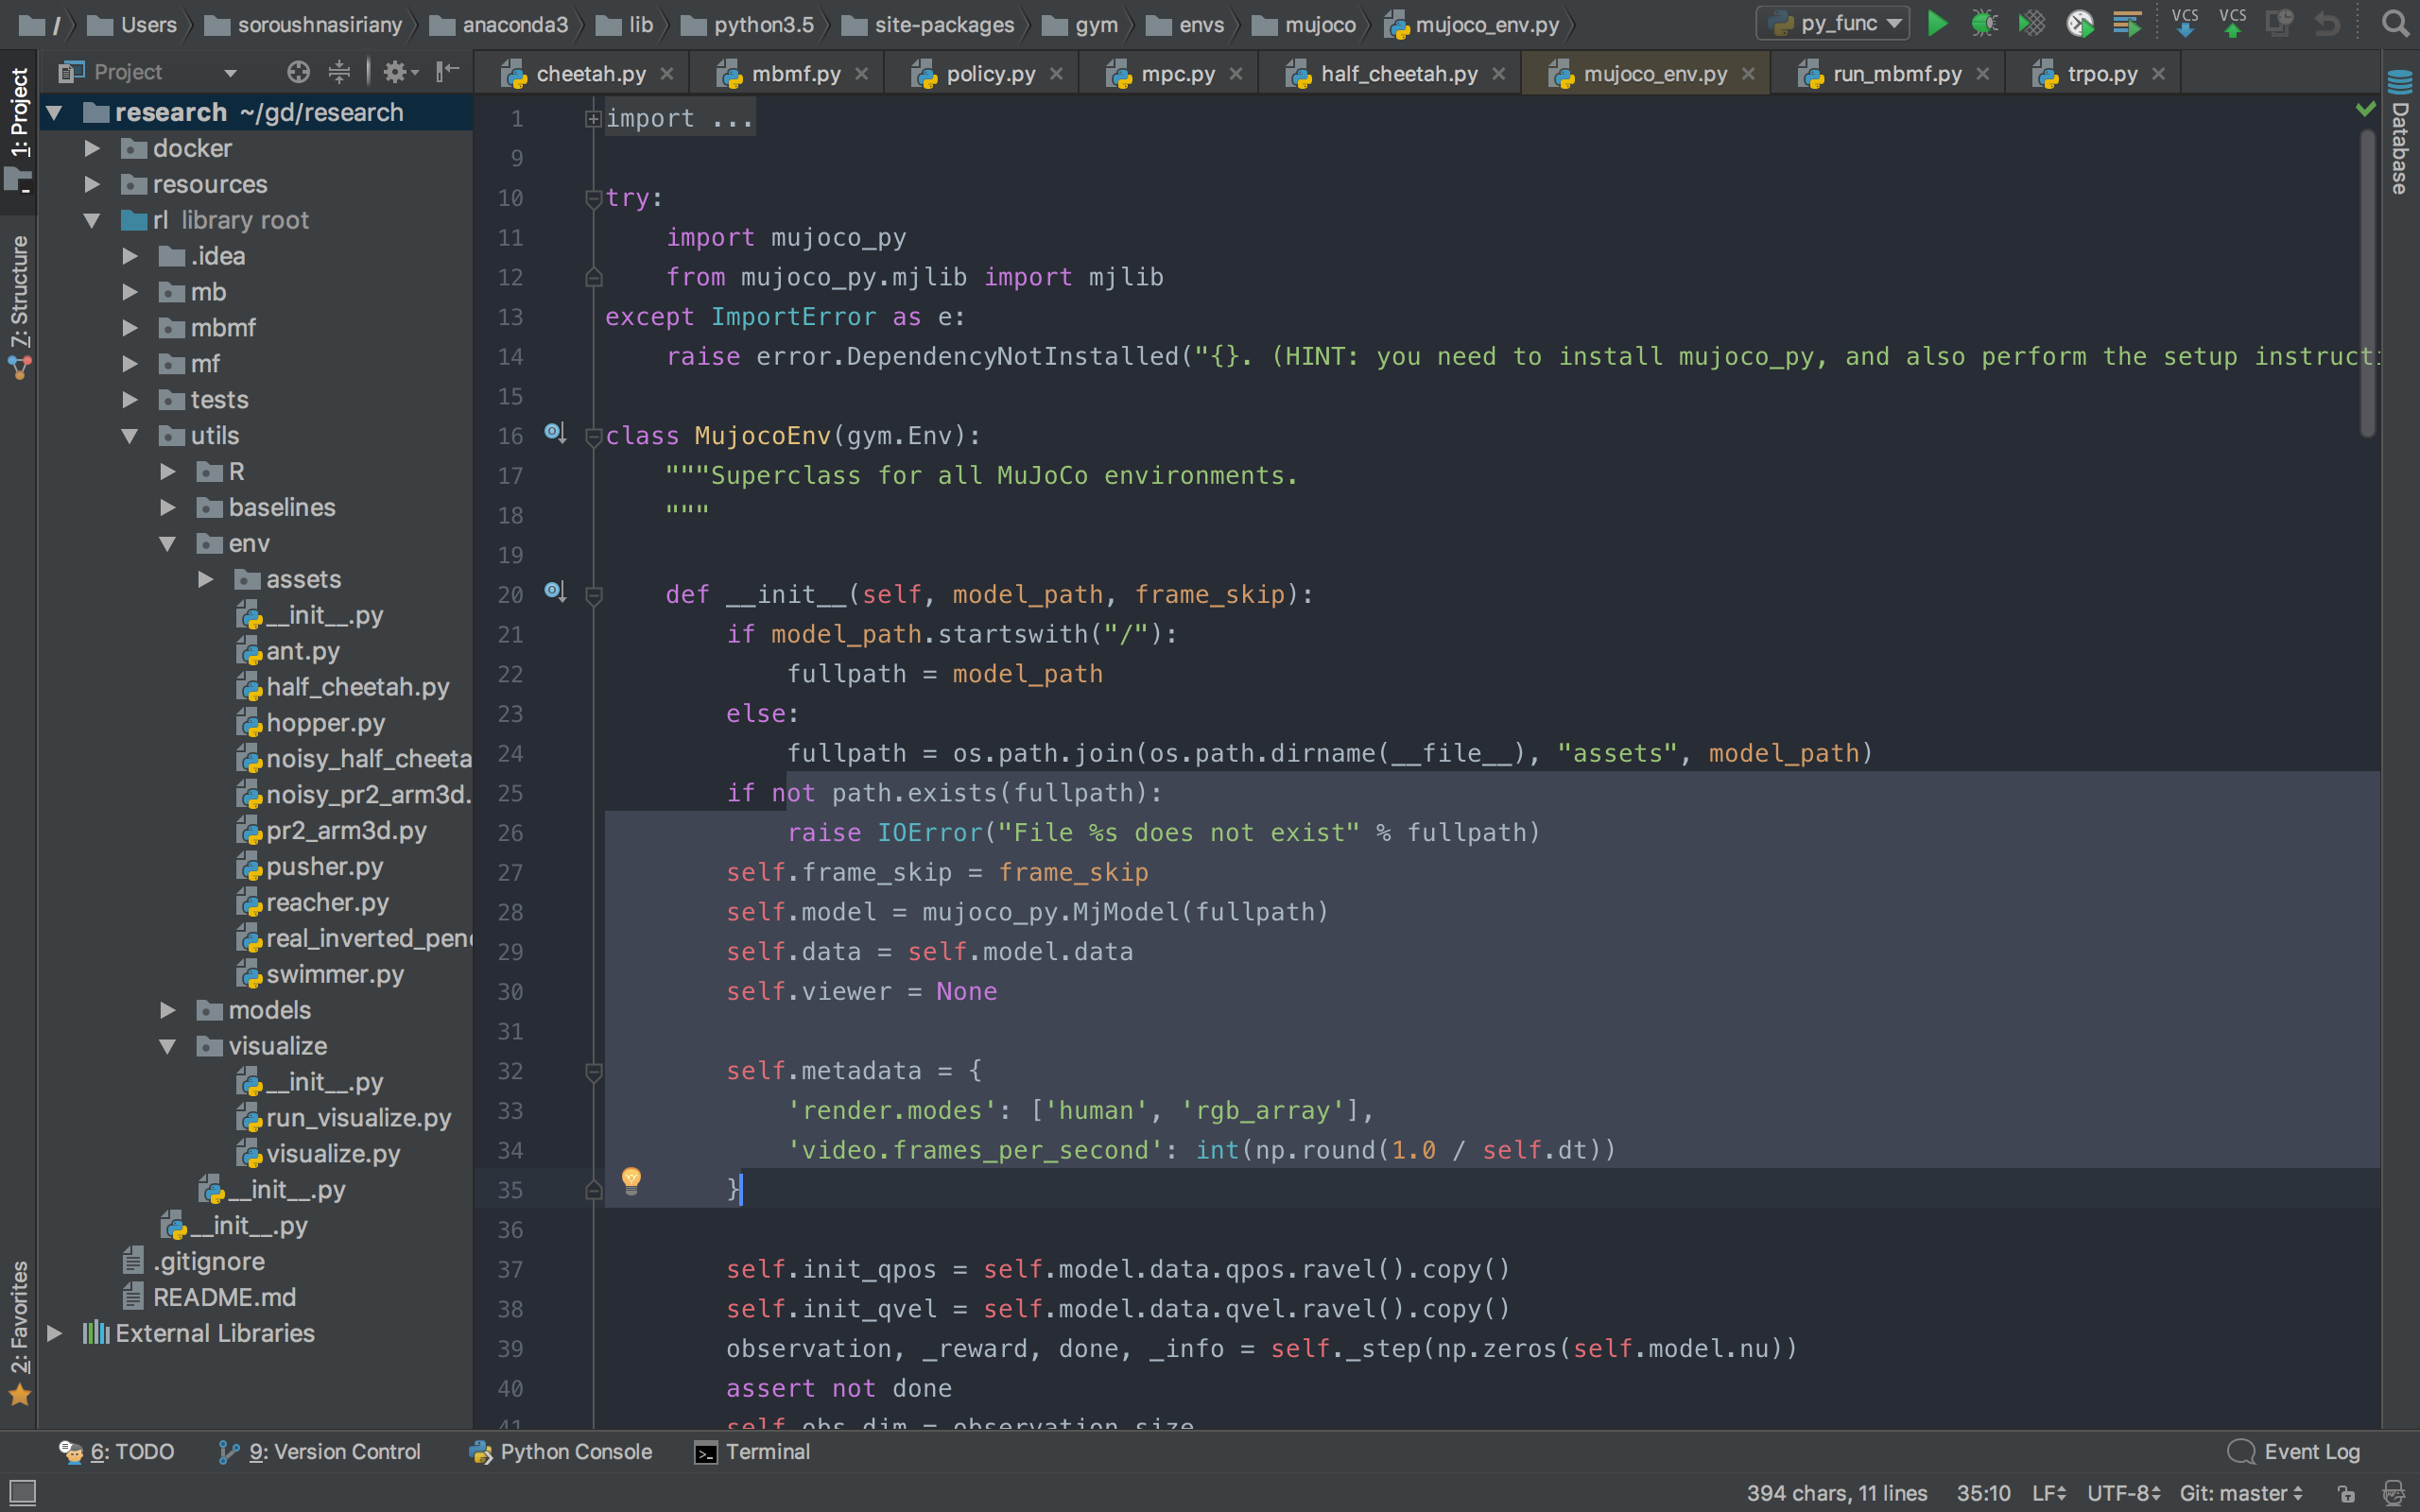
\includegraphics[width=\textwidth]{img/pycharm.png}
			\caption{Interfaccia grafica di PyCharm}
		\end{figure}
